\section{Part B}
%=========================Intro====================================%
So far the characterization of the graphics card performance was in terms of the speed of operations. Now we turn to characterize the quality, specifically the arithmetic precision. This is considered a crucial since the speed render irrelevant if the results are not accurate. Even under the IEEE-754 Standards, identical operations could produce different results when operated on two different machines (e.g. floating point addition is not associative). 

In this section, we start by quantifying the error of the basic arithmetic operations offered by OpenGL. We compare GPU's results with the CPU to measure the error. We also try to discover a precision-related undocumented features; how rounding is implemented in our graphic card. 

%=========================Arithmetic Opt====================================%
\subsection{Arithmetic Operations Accuracy:}
Here we test a range of basic arithmetic operation offered by OpenGL and GLSL. Taking the CPU results as our datum, the absolute relative error between the GPU's results and CPU's results represents the GPU errors. The rationale behind this method is that both CPU and GPU are compliant with IEEE-754 Standard. %We will revisit this idea in Section \ref{sec:dot}, where we see careful implementation could make the graphic card more accurate. 

%=========================Dot Product====================================%
%\subsection{Dot Product}\label{sec:dot}
%Here we performance dot product between two float vectors and measure the error between the 
%\cite{whitehead2011precision}

%=========================Rounding====================================%
\subsection{Rounding}
The purpose of this test is to first verify that our GPU is IEEE-754 compliant and second to identify the rounding algorithm implemented. For this test, we borrowed the fragment shader used in Russell's article \cite{stuart2013mobile} shown in Figure \ref{fig:shader1}. In Russell's article, the shader was used to benchmark the accuracy of GPU floating point across different mobile GPUs. 

The shader simply fills the screen with 26 bars. Given infinite precision, each bar should vary linearly from white (left) to black (right) as a function of $X$ coordinate of the pixel. The shader is written such that with each level/bar, one bit of the fraction is thrown away. For each level $L$, we add $2^{L}$ to the computed gray value ($X$ coordinate of the pixel) and take the fraction of the result. The added integer ($2^{L}$) does not affect the value of the gray scale, but only its precision. For example, for the first bar, we add  $2^{L}=(1)_{ten}=(1)_{two}$ which is represented by one bit. Thus, when added to $fract(x)$ and taking the $fract()$ of the result, we only loss one bit of the $x$ precision. For the next level, we add $2^{L}=(4)_{ten}=(10)_{two}$, which is represented by two bits and thus two bits loss in $x$ precision. This goes up till we end up with zero precision in the fraction part and thus the image turns to black. Figure \ref{fig:prec} shows the result of running the shader on our graphic card. We can see that even though we are trying to draw 26 bars, only 23 bars are shown and the rest are black. This verifies that the fraction part of float in our graphic card is represented by 23 bits which matches exactly what IEEE-754 requirements. 

\begin{figure}[t!]
\centering
\begin{minipage}[t]{\textwidth}
\centering
\begin{lstlisting}[label=list:ExampleShader,
escapechar=|,
caption={
  Fragment Shader.
}]
void main(void) {
  float y = (gl_FragCoord.y / 600) * 26.0
  float x = (1.0 -(gl_FragCoord.x / 800))
  float yp = pow(2.0, floor(y))
  float fade = fract(yp + fract(x))
  if (fract(y) < 0.9)
     gl_FragColor = vec4(vec3(fade), 1.0)
  else
     gl_FragColor = vec4(0.0)
}
|
\end{lstlisting}
\end{minipage}

\caption{The fragment shader implementation for verify the floating-point representation compliance with IEEE-754 standards}
\label{fig:shader1}
\end{figure}


\begin{figure}[t!]
 \centering   
 \subfloat[Precision Shader]
    {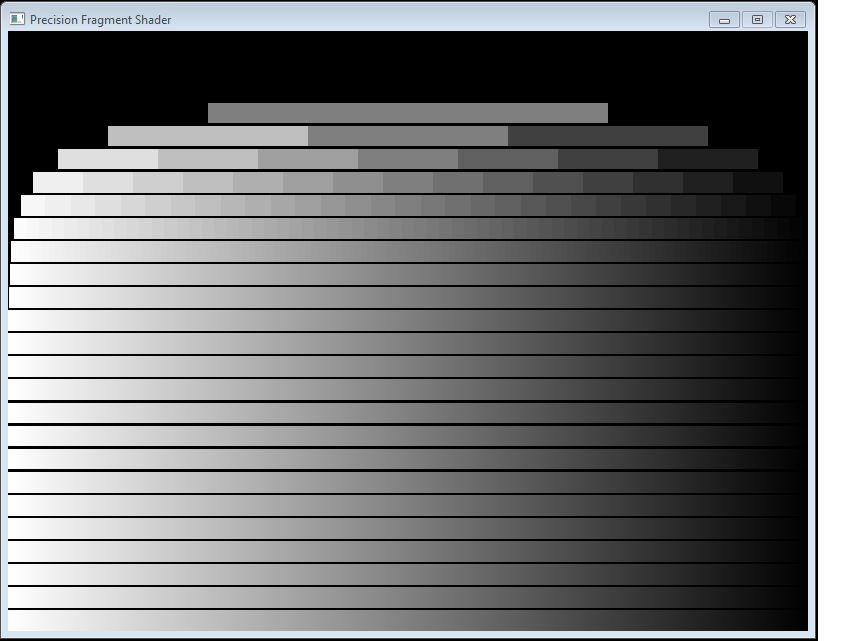
\includegraphics[width=0.49\linewidth]{fig/shader.JPG}} 
 \subfloat[blah]
   {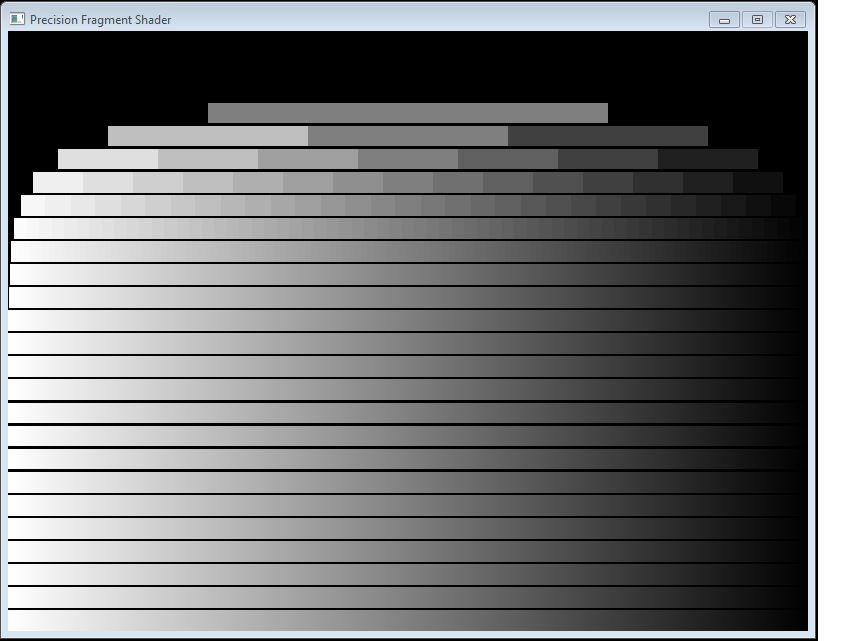
\includegraphics[width=0.49\linewidth]{fig/shader.JPG}}   
  \caption{Results of applying shader in Figure \ref{fig:shader1}  on our graphic card.}
   \label{fig:prec}
\end{figure} 





